% Options for packages loaded elsewhere
% Options for packages loaded elsewhere
\PassOptionsToPackage{unicode}{hyperref}
\PassOptionsToPackage{hyphens}{url}
\PassOptionsToPackage{dvipsnames,svgnames,x11names}{xcolor}
%
\documentclass[
  letterpaper,
  DIV=11,
  numbers=noendperiod]{scrartcl}
\usepackage{xcolor}
\usepackage{amsmath,amssymb}
\setcounter{secnumdepth}{5}
\usepackage{iftex}
\ifPDFTeX
  \usepackage[T1]{fontenc}
  \usepackage[utf8]{inputenc}
  \usepackage{textcomp} % provide euro and other symbols
\else % if luatex or xetex
  \usepackage{unicode-math} % this also loads fontspec
  \defaultfontfeatures{Scale=MatchLowercase}
  \defaultfontfeatures[\rmfamily]{Ligatures=TeX,Scale=1}
\fi
\usepackage{lmodern}
\ifPDFTeX\else
  % xetex/luatex font selection
\fi
% Use upquote if available, for straight quotes in verbatim environments
\IfFileExists{upquote.sty}{\usepackage{upquote}}{}
\IfFileExists{microtype.sty}{% use microtype if available
  \usepackage[]{microtype}
  \UseMicrotypeSet[protrusion]{basicmath} % disable protrusion for tt fonts
}{}
\makeatletter
\@ifundefined{KOMAClassName}{% if non-KOMA class
  \IfFileExists{parskip.sty}{%
    \usepackage{parskip}
  }{% else
    \setlength{\parindent}{0pt}
    \setlength{\parskip}{6pt plus 2pt minus 1pt}}
}{% if KOMA class
  \KOMAoptions{parskip=half}}
\makeatother
% Make \paragraph and \subparagraph free-standing
\makeatletter
\ifx\paragraph\undefined\else
  \let\oldparagraph\paragraph
  \renewcommand{\paragraph}{
    \@ifstar
      \xxxParagraphStar
      \xxxParagraphNoStar
  }
  \newcommand{\xxxParagraphStar}[1]{\oldparagraph*{#1}\mbox{}}
  \newcommand{\xxxParagraphNoStar}[1]{\oldparagraph{#1}\mbox{}}
\fi
\ifx\subparagraph\undefined\else
  \let\oldsubparagraph\subparagraph
  \renewcommand{\subparagraph}{
    \@ifstar
      \xxxSubParagraphStar
      \xxxSubParagraphNoStar
  }
  \newcommand{\xxxSubParagraphStar}[1]{\oldsubparagraph*{#1}\mbox{}}
  \newcommand{\xxxSubParagraphNoStar}[1]{\oldsubparagraph{#1}\mbox{}}
\fi
\makeatother


\usepackage{longtable,booktabs,array}
\newcounter{none} % for unnumbered tables
\usepackage{calc} % for calculating minipage widths
% Correct order of tables after \paragraph or \subparagraph
\usepackage{etoolbox}
\makeatletter
\patchcmd\longtable{\par}{\if@noskipsec\mbox{}\fi\par}{}{}
\makeatother
% Allow footnotes in longtable head/foot
\IfFileExists{footnotehyper.sty}{\usepackage{footnotehyper}}{\usepackage{footnote}}
\makesavenoteenv{longtable}
\usepackage{graphicx}
\makeatletter
\newsavebox\pandoc@box
\newcommand*\pandocbounded[1]{% scales image to fit in text height/width
  \sbox\pandoc@box{#1}%
  \Gscale@div\@tempa{\textheight}{\dimexpr\ht\pandoc@box+\dp\pandoc@box\relax}%
  \Gscale@div\@tempb{\linewidth}{\wd\pandoc@box}%
  \ifdim\@tempb\p@<\@tempa\p@\let\@tempa\@tempb\fi% select the smaller of both
  \ifdim\@tempa\p@<\p@\scalebox{\@tempa}{\usebox\pandoc@box}%
  \else\usebox{\pandoc@box}%
  \fi%
}
% Set default figure placement to htbp
\def\fps@figure{htbp}
\makeatother


% definitions for citeproc citations
\NewDocumentCommand\citeproctext{}{}
\NewDocumentCommand\citeproc{mm}{%
  \begingroup\def\citeproctext{#2}\cite{#1}\endgroup}
\makeatletter
 % allow citations to break across lines
 \let\@cite@ofmt\@firstofone
 % avoid brackets around text for \cite:
 \def\@biblabel#1{}
 \def\@cite#1#2{{#1\if@tempswa , #2\fi}}
\makeatother
\newlength{\cslhangindent}
\setlength{\cslhangindent}{1.5em}
\newlength{\csllabelwidth}
\setlength{\csllabelwidth}{3em}
\newenvironment{CSLReferences}[2] % #1 hanging-indent, #2 entry-spacing
 {\begin{list}{}{%
  \setlength{\itemindent}{0pt}
  \setlength{\leftmargin}{0pt}
  \setlength{\parsep}{0pt}
  % turn on hanging indent if param 1 is 1
  \ifodd #1
   \setlength{\leftmargin}{\cslhangindent}
   \setlength{\itemindent}{-1\cslhangindent}
  \fi
  % set entry spacing
  \setlength{\itemsep}{#2\baselineskip}}}
 {\end{list}}
\usepackage{calc}
\newcommand{\CSLBlock}[1]{\hfill\break\parbox[t]{\linewidth}{\strut\ignorespaces#1\strut}}
\newcommand{\CSLLeftMargin}[1]{\parbox[t]{\csllabelwidth}{\strut#1\strut}}
\newcommand{\CSLRightInline}[1]{\parbox[t]{\linewidth - \csllabelwidth}{\strut#1\strut}}
\newcommand{\CSLIndent}[1]{\hspace{\cslhangindent}#1}



\setlength{\emergencystretch}{3em} % prevent overfull lines

\providecommand{\tightlist}{%
  \setlength{\itemsep}{0pt}\setlength{\parskip}{0pt}}



 


\KOMAoption{captions}{tableheading}
\makeatletter
\@ifpackageloaded{caption}{}{\usepackage{caption}}
\AtBeginDocument{%
\ifdefined\contentsname
  \renewcommand*\contentsname{Table of contents}
\else
  \newcommand\contentsname{Table of contents}
\fi
\ifdefined\listfigurename
  \renewcommand*\listfigurename{List of Figures}
\else
  \newcommand\listfigurename{List of Figures}
\fi
\ifdefined\listtablename
  \renewcommand*\listtablename{List of Tables}
\else
  \newcommand\listtablename{List of Tables}
\fi
\ifdefined\figurename
  \renewcommand*\figurename{Figure}
\else
  \newcommand\figurename{Figure}
\fi
\ifdefined\tablename
  \renewcommand*\tablename{Table}
\else
  \newcommand\tablename{Table}
\fi
}
\@ifpackageloaded{float}{}{\usepackage{float}}
\floatstyle{ruled}
\@ifundefined{c@chapter}{\newfloat{codelisting}{h}{lop}}{\newfloat{codelisting}{h}{lop}[chapter]}
\floatname{codelisting}{Listing}
\newcommand*\listoflistings{\listof{codelisting}{List of Listings}}
\makeatother
\makeatletter
\makeatother
\makeatletter
\@ifpackageloaded{caption}{}{\usepackage{caption}}
\@ifpackageloaded{subcaption}{}{\usepackage{subcaption}}
\makeatother
\usepackage{bookmark}
\IfFileExists{xurl.sty}{\usepackage{xurl}}{} % add URL line breaks if available
\urlstyle{same}
\hypersetup{
  pdftitle={Careless/Insufficient Effort Responding (C/IER) Detection},
  pdfauthor={Pablo Rogers},
  pdfkeywords={Careless Responding, Insufficient Effort
Responding, Laz.R, Longstring, Mahalanobis Distance, IRV},
  colorlinks=true,
  linkcolor={blue},
  filecolor={Maroon},
  citecolor={Blue},
  urlcolor={Blue},
  pdfcreator={LaTeX via pandoc}}


\title{Careless/Insufficient Effort Responding (C/IER) Detection}
\author{Pablo Rogers}
\date{2026-04-03}
\begin{document}
\maketitle
\begin{abstract}
This notebook presents a tutorial on the detection of careless or
insufficient effort responding (C/IER) in self-report questionnaires. We
use real database from WHOQOL-Bref scale as an example (n = 1,546), and
we apply the `careless' package and Laz.R (Biemann et al., 2025) to
detect C/IER (post hoc indicators). We also discuss the importance of
procedural C/IER detection in the quality control of data obtained
through self-report questionnaires.
\end{abstract}


\section{Contextualization}\label{contextualization}

The detection of Careless or Insufficient Effort Responding (C/IER) is
an essential step in the quality control of data obtained through
self-report questionnaires. C/IER occurs when respondents complete the
instrument without attention to the item content, compromising the
validity of the psychometric and substantive inferences derived from the
data (Curran, 2016; Huang et al., 2026).

The analytical flow of this document follows two sequential levels of
detection:

\begin{enumerate}
\def\labelenumi{\arabic{enumi}.}
\tightlist
\item
  \textbf{Questionnaire:} procedural exclusions (a priori), including
  dropout, response time, and quality control items.
\item
  \textbf{WHOQOL Scale:} diagnostic post-hoc indicators (Laz.R,
  Longstring, Mahalanobis Distance, and IRV) with cut-off points
  estimated via the Kneedle algorithm (Biemann et al., 2025).
\end{enumerate}

\section{Data reading and
preparation}\label{data-reading-and-preparation}

The \texttt{data.csv} file contains the raw survey responses (separator
\texttt{;}). In this step, dropout records are removed, variables for
the analytical flow are selected, and the total response time
(\texttt{TIME}) is derived.

\protect\phantomsection\label{data-reading}
\begin{longtable}[]{@{}
  >{\raggedright\arraybackslash}p{(\linewidth - 6\tabcolsep) * \real{0.2125}}
  >{\raggedright\arraybackslash}p{(\linewidth - 6\tabcolsep) * \real{0.1750}}
  >{\raggedright\arraybackslash}p{(\linewidth - 6\tabcolsep) * \real{0.1750}}
  >{\raggedright\arraybackslash}p{(\linewidth - 6\tabcolsep) * \real{0.4125}}@{}}
\caption{Structure and variable dictionary of the prepared survey
dataset (\protect\texttt{imported\_data})}\tabularnewline
\toprule\noalign{}
\begin{minipage}[b]{\linewidth}\raggedright
Group
\end{minipage} & \begin{minipage}[b]{\linewidth}\raggedright
Variables
\end{minipage} & \begin{minipage}[b]{\linewidth}\raggedright
Class / Type
\end{minipage} & \begin{minipage}[b]{\linewidth}\raggedright
Description
\end{minipage} \\
\midrule\noalign{}
\endfirsthead
\toprule\noalign{}
\begin{minipage}[b]{\linewidth}\raggedright
Group
\end{minipage} & \begin{minipage}[b]{\linewidth}\raggedright
Variables
\end{minipage} & \begin{minipage}[b]{\linewidth}\raggedright
Class / Type
\end{minipage} & \begin{minipage}[b]{\linewidth}\raggedright
Description
\end{minipage} \\
\midrule\noalign{}
\endhead
\bottomrule\noalign{}
\endlastfoot
Identification & ID & Numeric (Double) & Unique respondent identifier \\
Timing & CREATED, MODIFIED, TIME & Date-time / Numeric (s) & Survey
timestamps and total response duration in seconds \\
Attention Checks & CQ1, CQ2, CQ3 & Binary (0/1) & Quality control check
items (1 = passed, 0 = failed) \\
WHOQOL-Bref Scale & Q1 to Q26 (26 items) & Ordinal (1 to 5) &
Self-reported quality of life items \\
\end{longtable}

\textsubscript{Source:
\href{https://phdpablo.github.io/cier/Scripts/ProcessingScripts/01_procedural-preview.html\#cell-data-reading}{Procedural
exclusions}}

\section{Procedural exclusions}\label{procedural-exclusions}

Level 1 applies three procedures prior to calculating post-hoc
indicators: dropout removal, exclusion for response time below 208
seconds (104 items × 2 s/item) (Huang et al., 2026), and exclusion for
two or more failures on quality control items (\texttt{CQ1-CQ3})
(Curran, 2016). Every exclusion is recorded in
\texttt{exclusion\_log.csv} with its reason and criterion.

{

\begin{longtable}[]{@{}lr@{}}

\caption{\label{tbl-level-1-summary}Procedural exclusions summary}

\tabularnewline

\toprule\noalign{}
Step & N \\
\midrule\noalign{}
\endhead
\bottomrule\noalign{}
\endlastfoot
Raw data & 1546 \\
Dropouts removed & 220 \\
Excluded by time (\textless{} 208 s) & 0 \\
Excluded by QC (≥ 2 fails) & 28 \\
Excluded by missings (\textgreater{} 5 in Q1-Q26) & 3 \\
Eligible for Level 2 & 1295 \\
Remaining NAs in Q1-Q26 & 90 \\

\end{longtable}

}

\textsubscript{Source:
\href{https://phdpablo.github.io/cier/Scripts/ProcessingScripts/01_procedural-preview.html\#cell-tbl-level-1-summary}{Procedural
exclusions}}

\section{Calculation of C/IER
indicators}\label{calculation-of-cier-indicators}

Each indicator captures distinct manifestations of C/IER; their
concurrent presence offers stronger evidence than any single indicator
alone (Curran, 2016; Hong et al., 2020; Huang et al., 2026).

\subsection{Univariate visualization}\label{univariate-visualization}

\begin{figure}[H]

\begin{minipage}[t]{0.50\linewidth}

\centering{

\pandocbounded{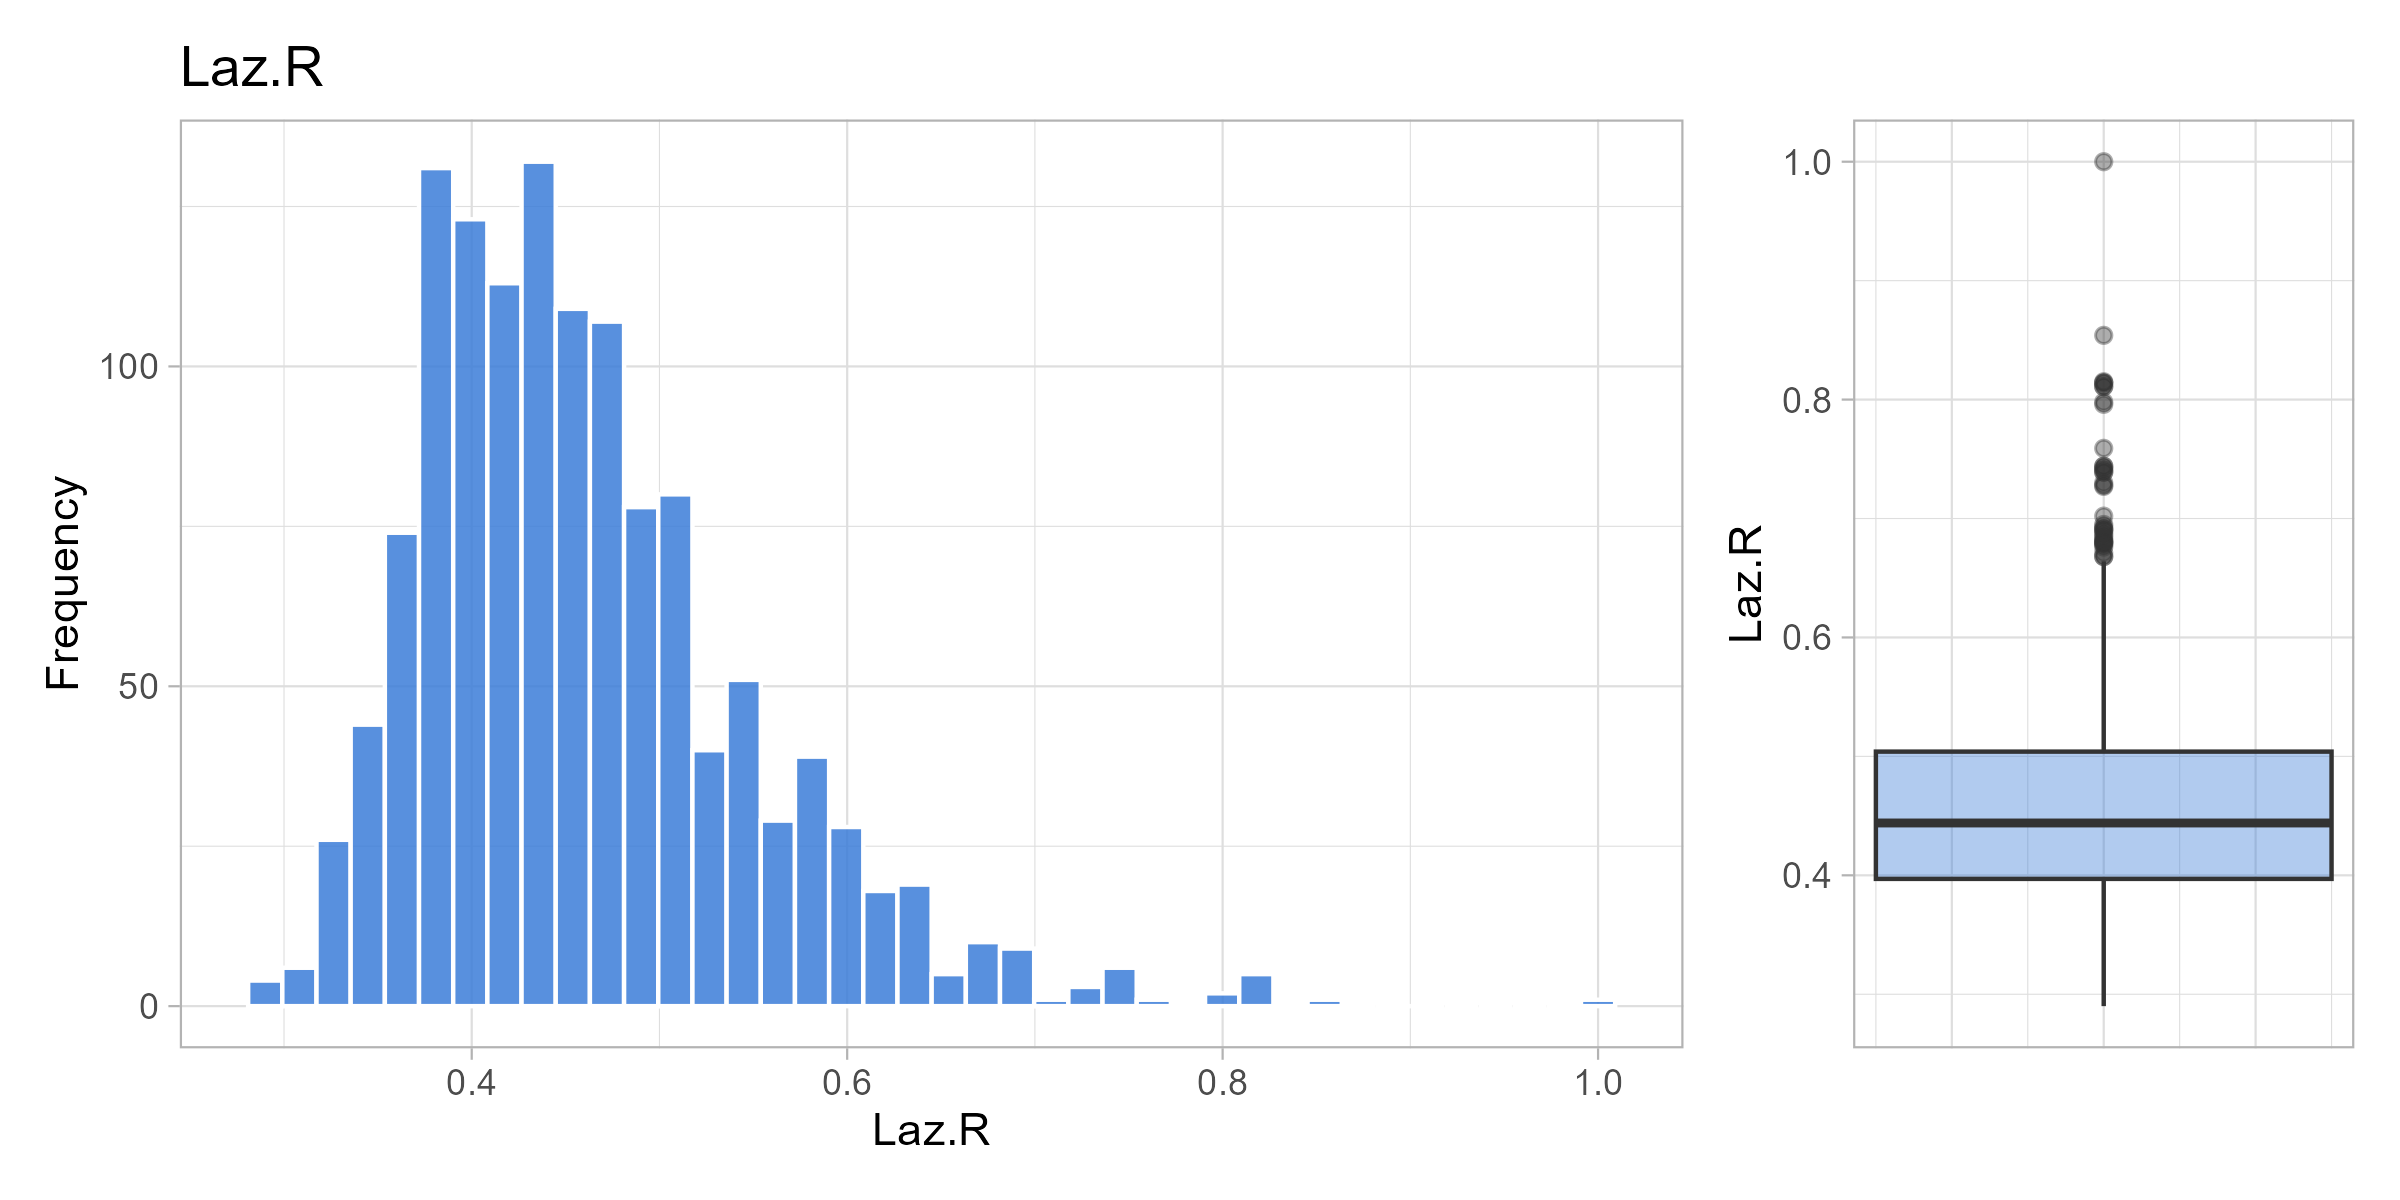
\includegraphics[keepaspectratio]{Output/Results/Figures/fig-viz-lazr.png}}

}

\subcaption{\label{fig-viz-lazr-pdf}Laz.R}

\end{minipage}%
%
\begin{minipage}[t]{0.50\linewidth}

\centering{

\pandocbounded{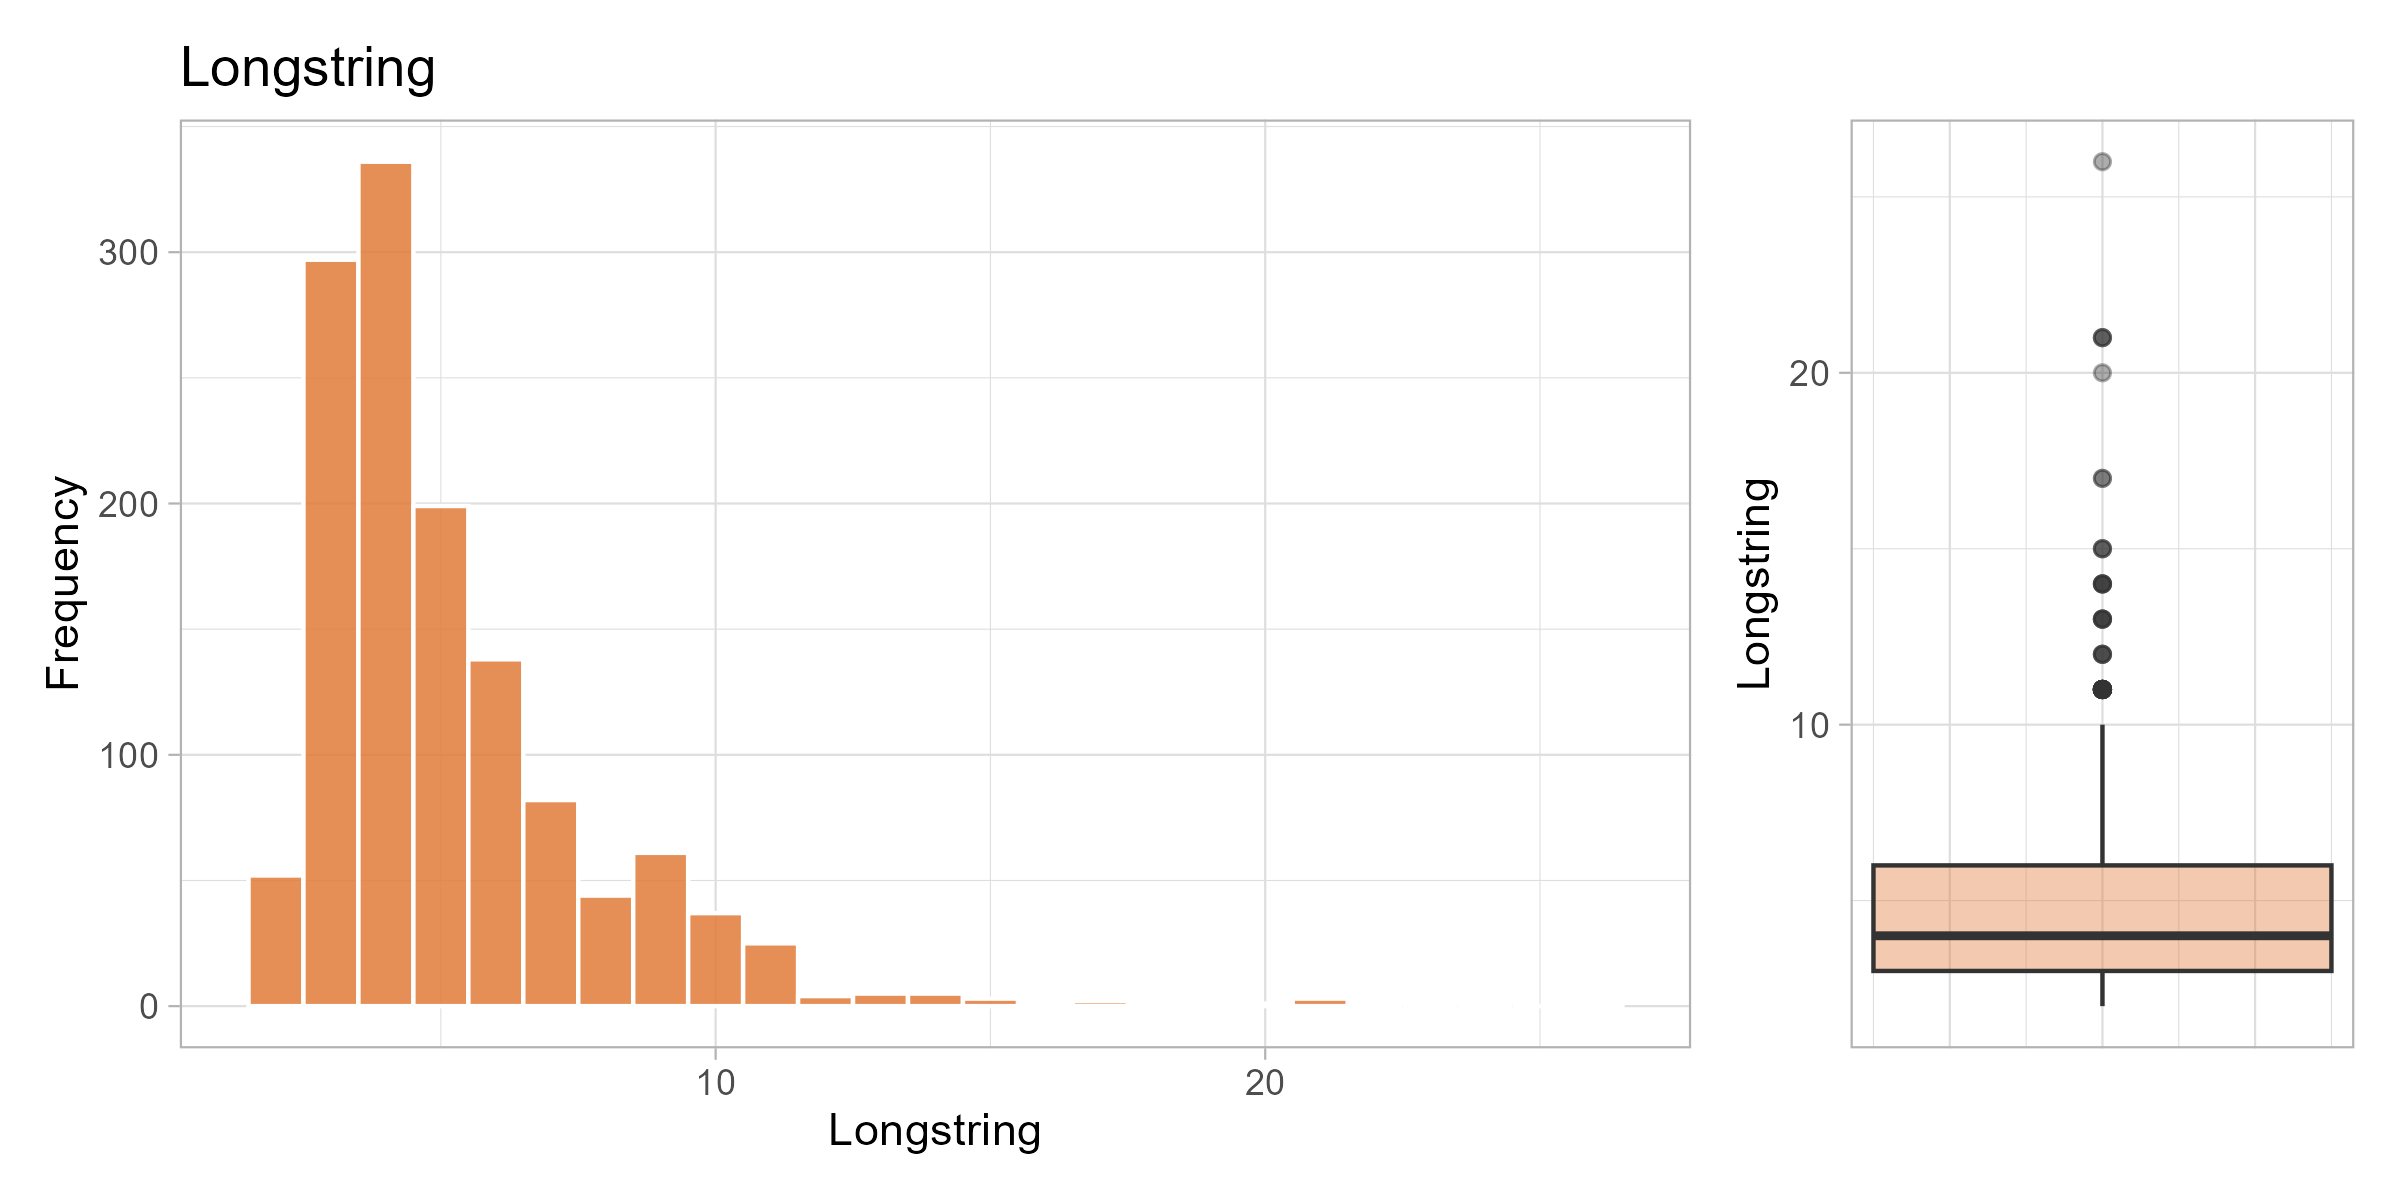
\includegraphics[keepaspectratio]{Output/Results/Figures/fig-viz-longstr.png}}

}

\subcaption{\label{fig-viz-longstr-pdf}Longstring}

\end{minipage}%
\newline
\begin{minipage}[t]{0.50\linewidth}

\centering{

\pandocbounded{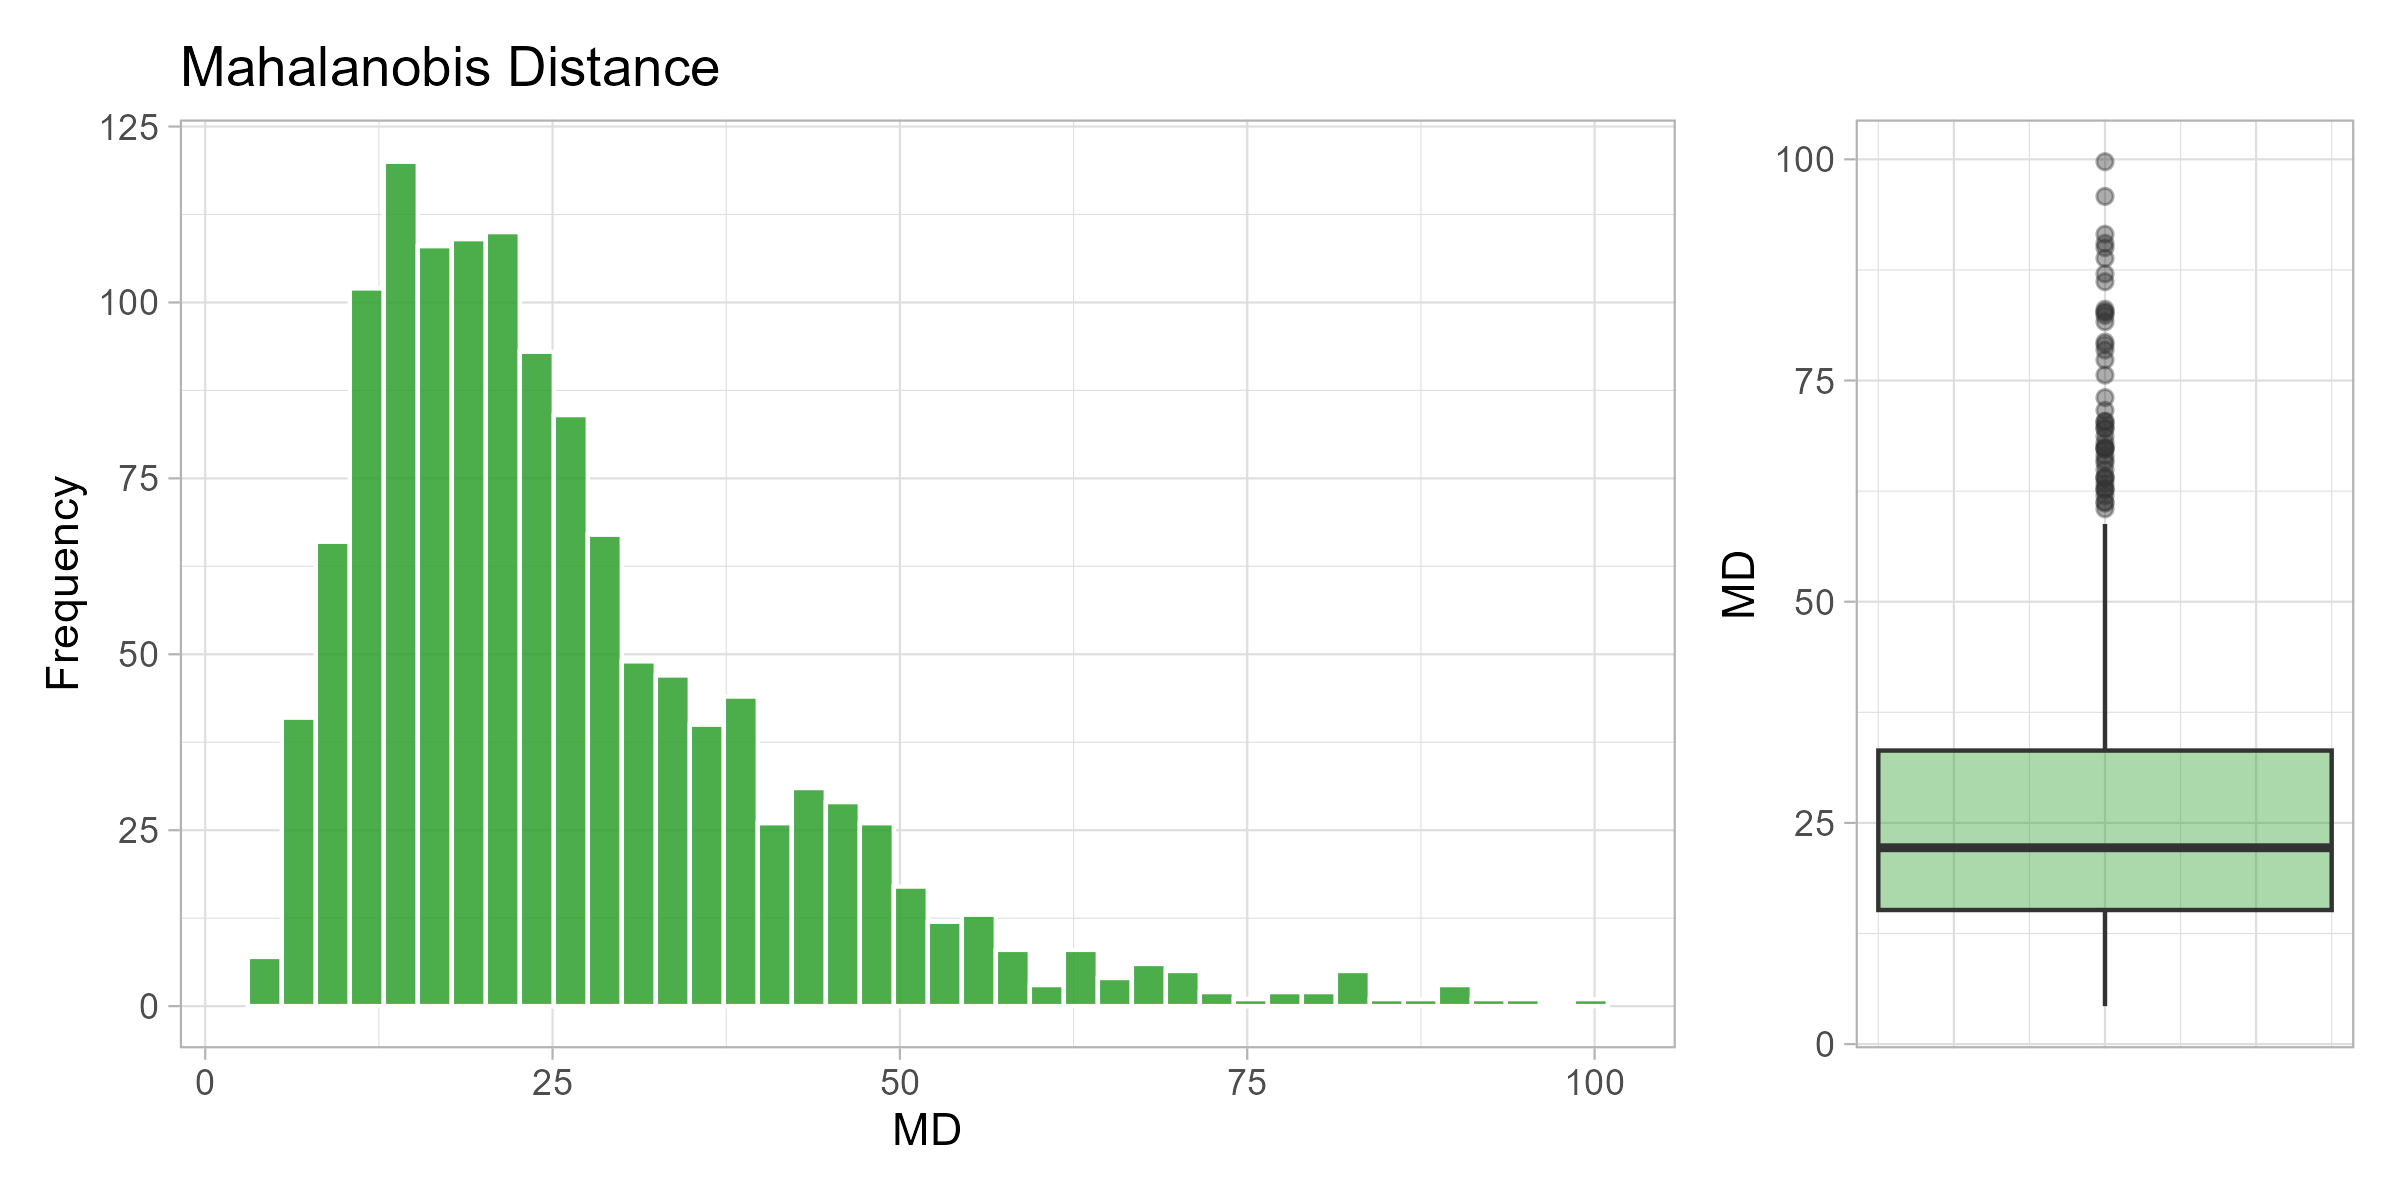
\includegraphics[keepaspectratio]{Output/Results/Figures/fig-viz-md.png}}

}

\subcaption{\label{fig-viz-md-pdf}Mahalanobis Distance}

\end{minipage}%
%
\begin{minipage}[t]{0.50\linewidth}

\centering{

\pandocbounded{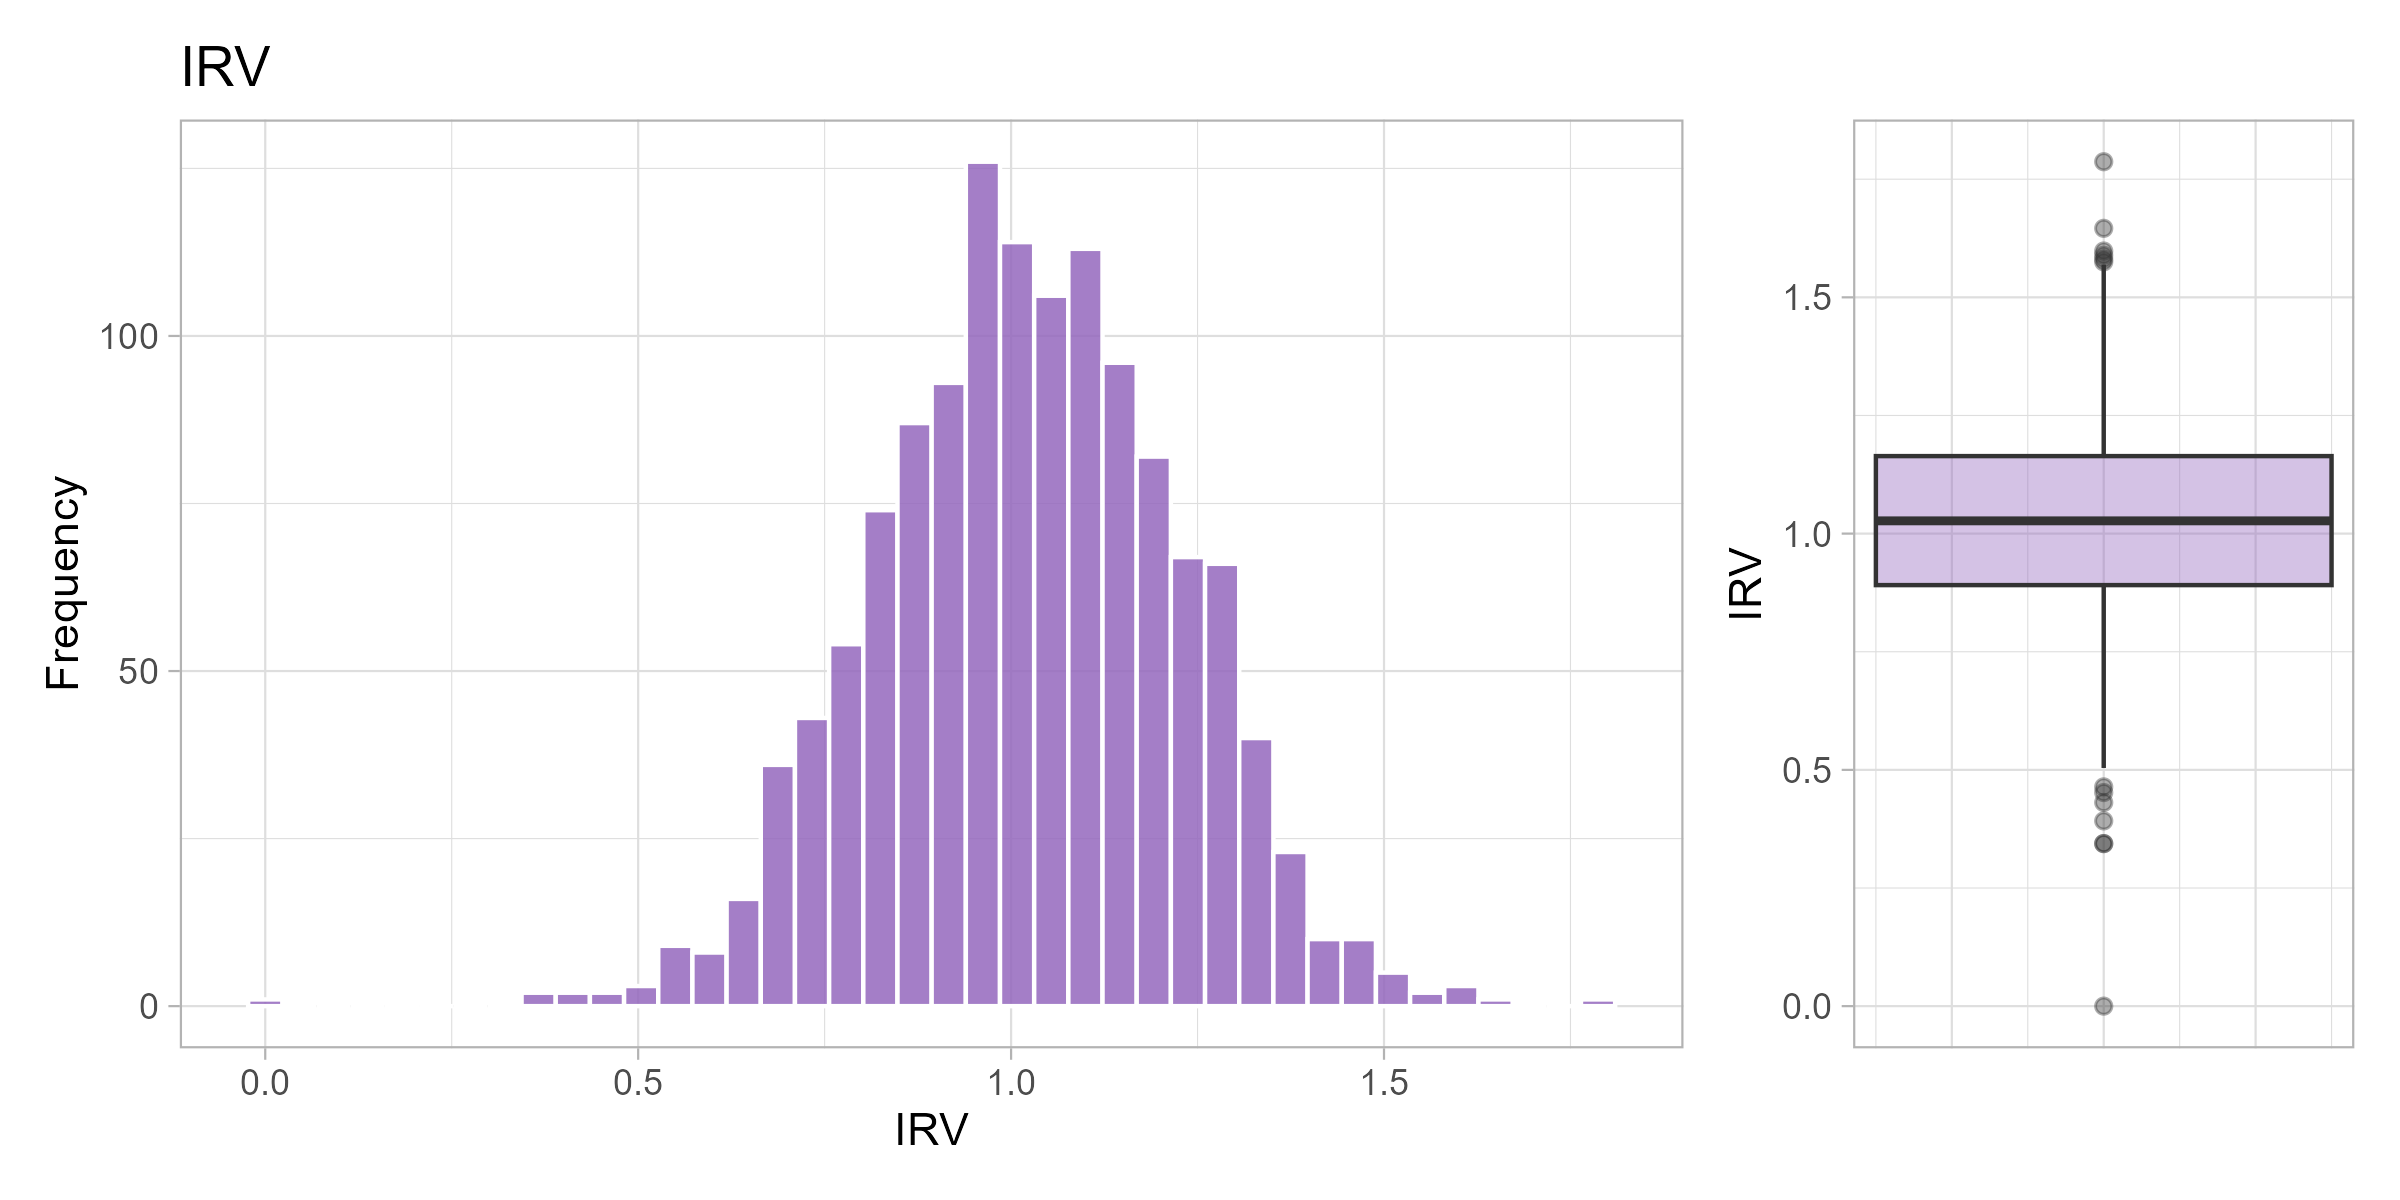
\includegraphics[keepaspectratio]{Output/Results/Figures/fig-viz-irv.png}}

}

\subcaption{\label{fig-viz-irv-pdf}IRV}

\end{minipage}%

\caption{\label{fig-univariate}Univariate distributions of C/IER
indicators}

\end{figure}%

\subsection{Cut-off points via Kneedle
algorithm}\label{cut-off-points-via-kneedle-algorithm}

The Kneedle algorithm is applied to the sorted (descending) curve of
each indicator. For \textbf{Laz.R}, \textbf{Longstring}, and
\textbf{MD}, kneedle with \texttt{sign\ =\ -1} identifies where
extremely high values separate from the majority (right tail). For
\textbf{IRV}, \texttt{sign\ =\ -1} is used to detect excessively high
IRV and \texttt{sign\ =\ +1} for excessively low IRV, since both
extremes can be considered suspicious.

{

\begin{longtable}[]{@{}lrr@{}}

\caption{\label{tbl-kneedle-cutoffs}Cut-off points estimated with the
Kneedle algorithm}

\tabularnewline

\toprule\noalign{}
Indicator & Critical value & \% flagged \\
\midrule\noalign{}
\endhead
\bottomrule\noalign{}
\endlastfoot
Laz.R & 0.60 & 6.8 \\
Longstring & 7.00 & 14.8 \\
MD & 40.12 & 15.4 \\
IRV (high end) & 1.34 & 4.9 \\
IRV (low end) & 0.69 & 3.8 \\

\end{longtable}

}

\textsubscript{Source:
\href{https://phdpablo.github.io/cier/Scripts/ProcessingScripts/02_posthoc-preview.html\#cell-tbl-kneedle-cutoffs}{Post-hoc
C/IER Indicators}}

\subsection{Plots with cut-off points}\label{plots-with-cut-off-points}

\begin{figure}[H]

\begin{minipage}[t]{0.50\linewidth}

\centering{

\pandocbounded{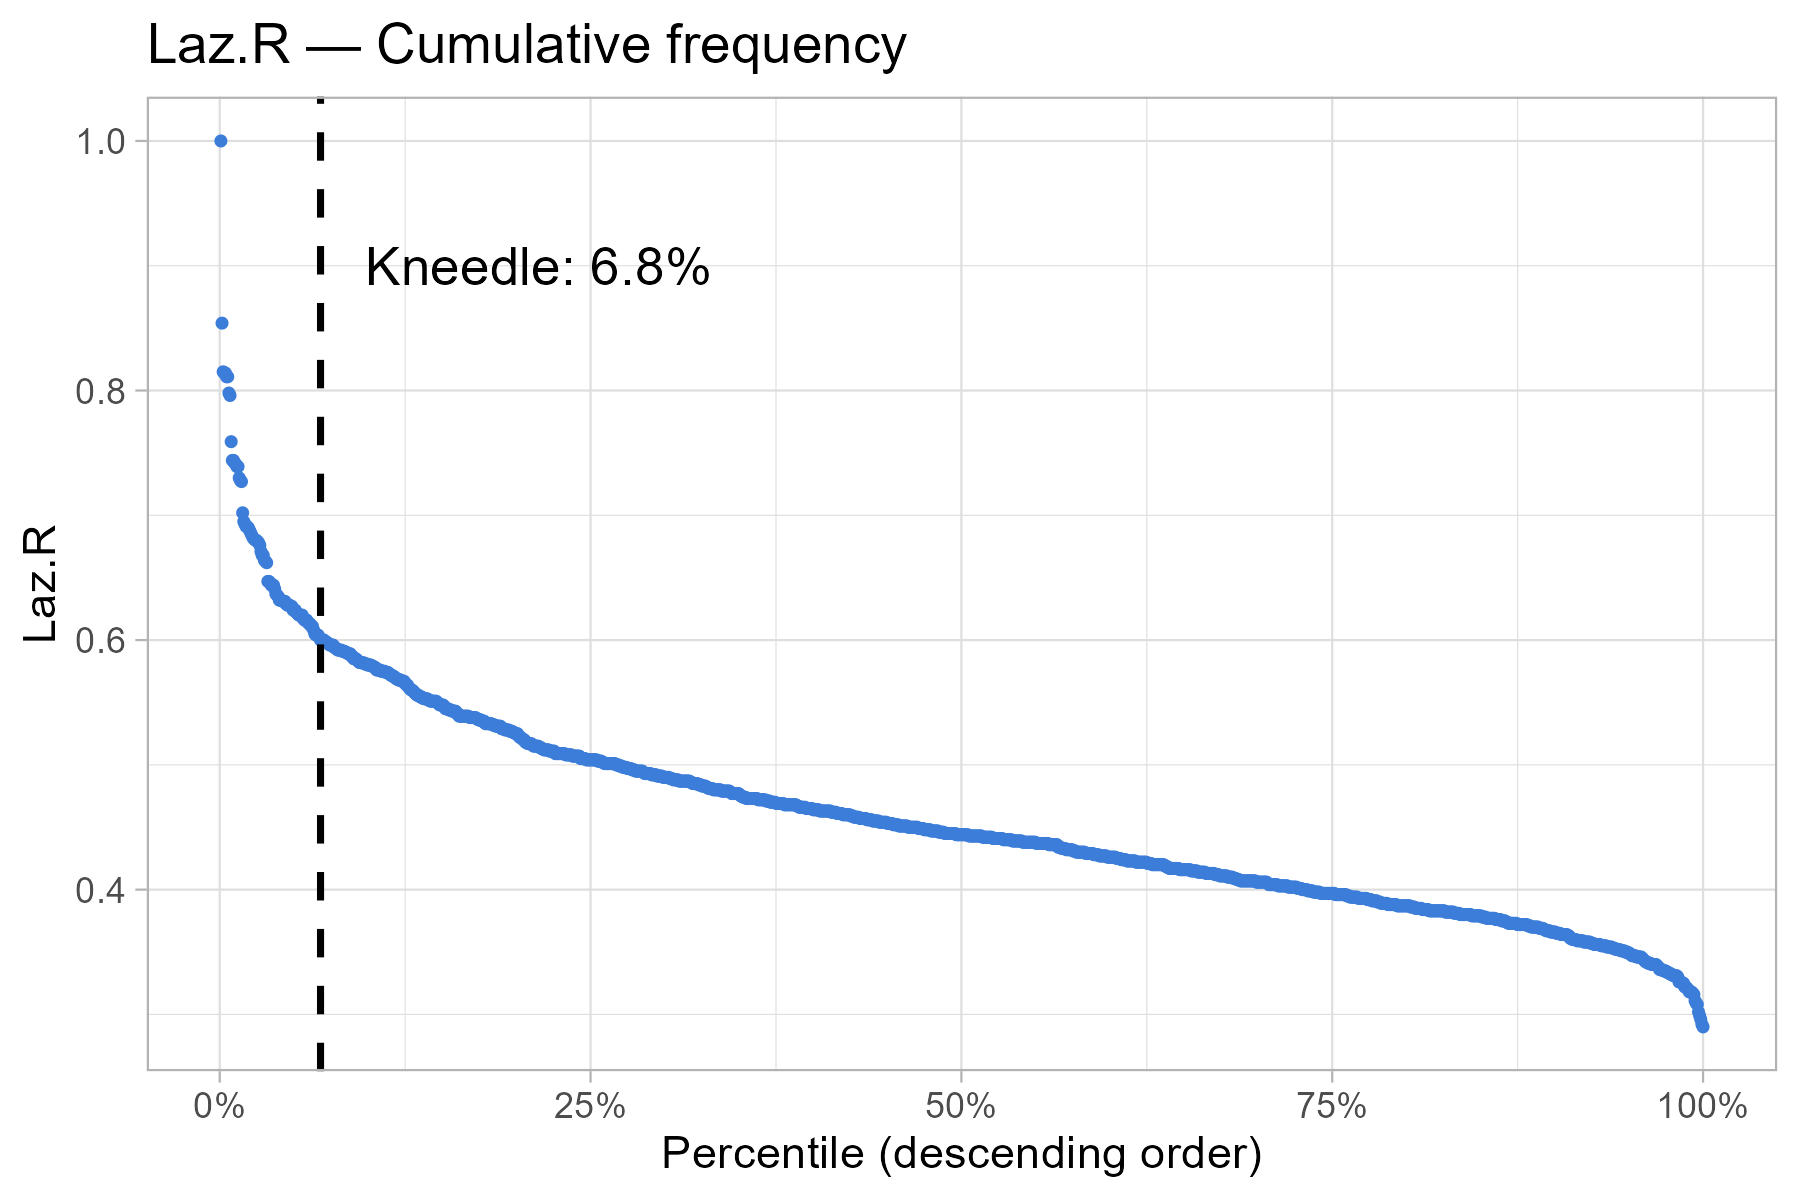
\includegraphics[keepaspectratio]{Output/Results/Figures/fig-cum-lazr.png}}

}

\subcaption{\label{fig-cum-lazr-pdf}Laz.R}

\end{minipage}%
%
\begin{minipage}[t]{0.50\linewidth}

\centering{

\pandocbounded{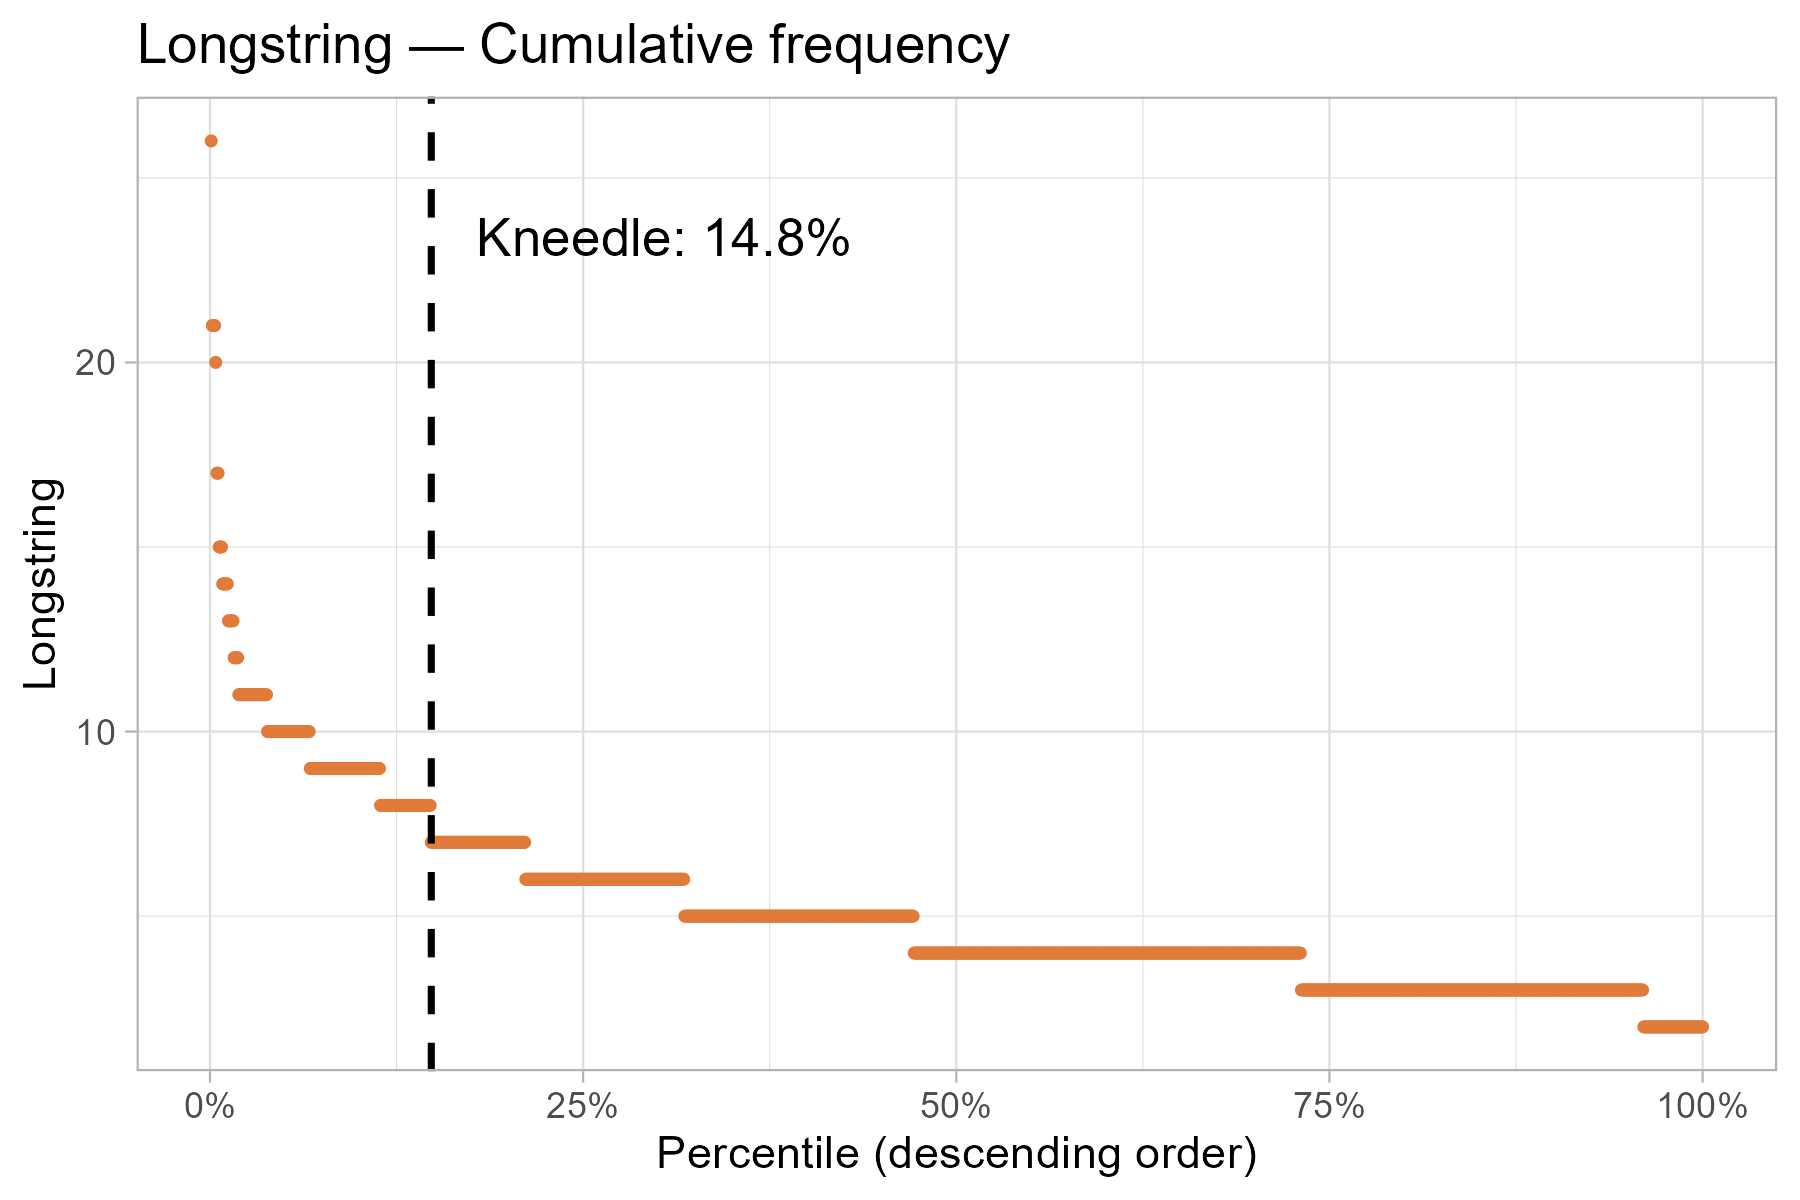
\includegraphics[keepaspectratio]{Output/Results/Figures/fig-cum-longstr.png}}

}

\subcaption{\label{fig-cum-longstr-pdf}Longstring}

\end{minipage}%
\newline
\begin{minipage}[t]{0.50\linewidth}

\centering{

\pandocbounded{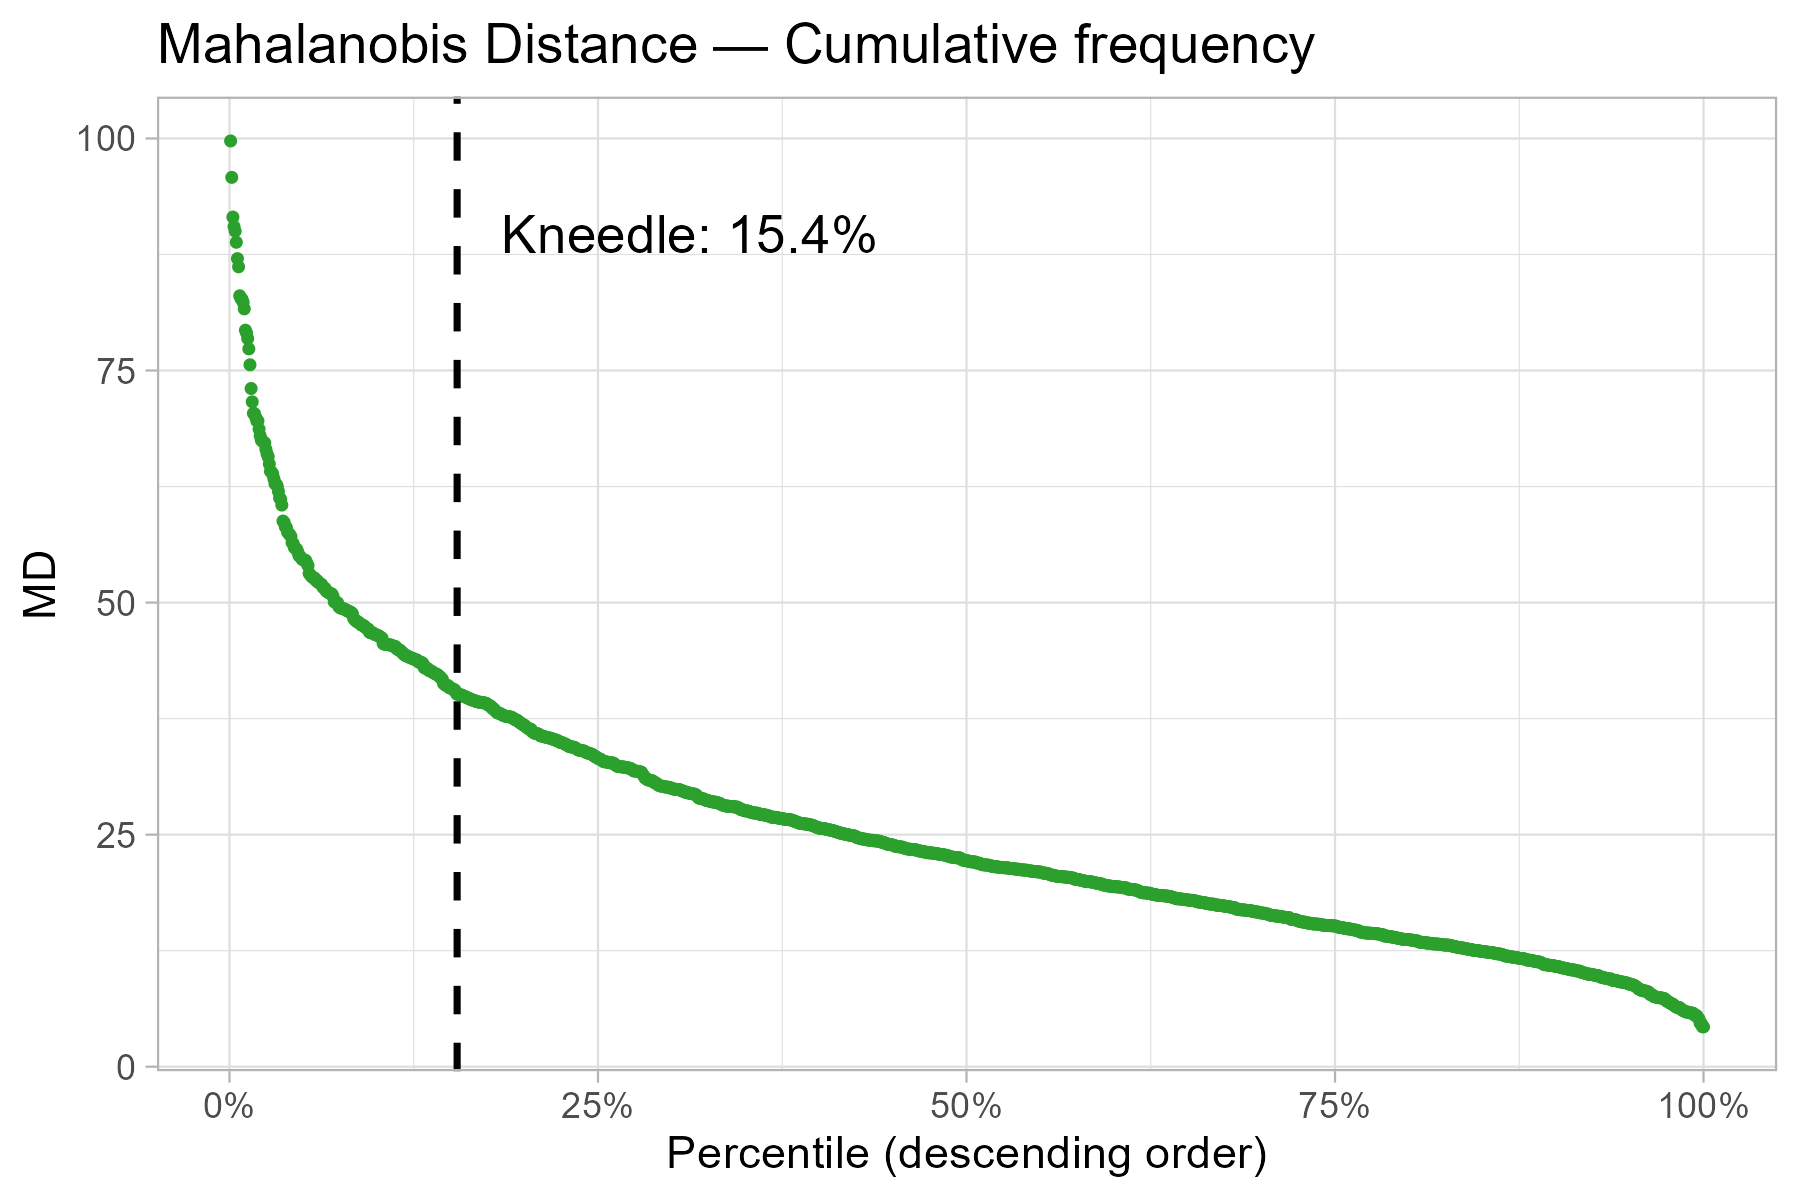
\includegraphics[keepaspectratio]{Output/Results/Figures/fig-cum-md.png}}

}

\subcaption{\label{fig-cum-md-pdf}Mahalanobis Distance}

\end{minipage}%
%
\begin{minipage}[t]{0.50\linewidth}

\centering{

\pandocbounded{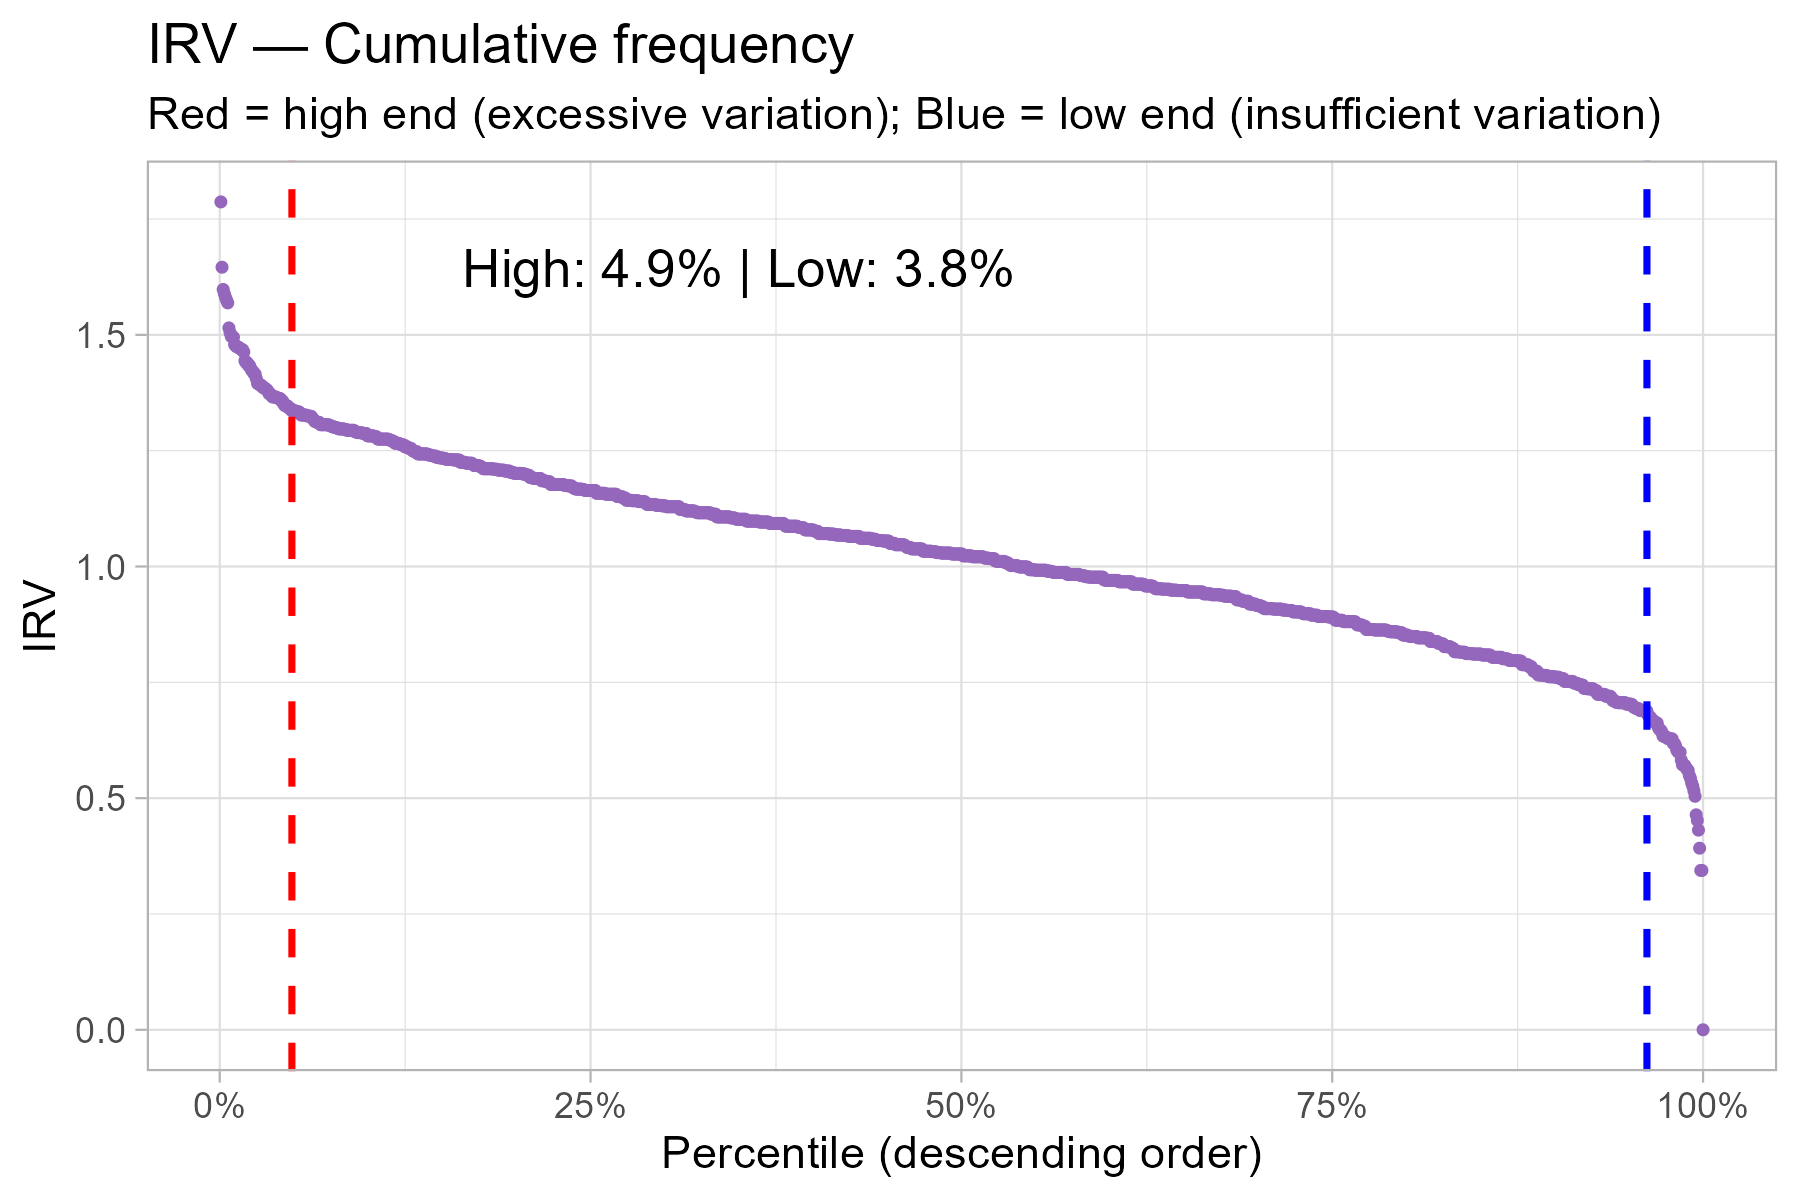
\includegraphics[keepaspectratio]{Output/Results/Figures/fig-cum-irv.png}}

}

\subcaption{\label{fig-cum-irv-pdf}IRV}

\end{minipage}%

\caption{\label{fig-cumulative}Cumulative frequency curves with Kneedle
cut-off points}

\end{figure}%

\subsection{C/IER Flags}\label{cier-flags}

For each indicator, a \texttt{\_FLAG} variable is created (\texttt{1} =
flagged, \texttt{0} = not flagged) based on the Kneedle cut-off points.

\begin{quote}
\textbf{Note:} Post-hoc indicators are \textbf{diagnostic}, they do not
trigger automatic exclusion in isolation. The final decision below
requires corroboration from at least two of four selected indicators.
\end{quote}

{

\begin{longtable}[]{@{}lrr@{}}

\caption{\label{tbl-flags-overview}Summary of respondents flagged by
each C/IER indicator}

\tabularnewline

\toprule\noalign{}
Indicator & N flagged & \% flagged \\
\midrule\noalign{}
\endhead
\bottomrule\noalign{}
\endlastfoot
LazR\_FLAG & 91 & 7.0 \\
Longstr\_FLAG & 191 & 14.7 \\
MD\_FLAG & 201 & 15.5 \\
IRV\_high\_FLAG & 66 & 5.1 \\
IRV\_low\_FLAG & 49 & 3.8 \\

\end{longtable}

}

\textsubscript{Source:
\href{https://phdpablo.github.io/cier/Scripts/ProcessingScripts/02_posthoc-preview.html\#cell-tbl-flags-overview}{Post-hoc
C/IER Indicators}}

\subsection{From diagnostic flags to final
exclusions}\label{posthoc-decision}

The cut-offs above identify response patterns that warrant attention;
they do not, by themselves, prove that a respondent answered carelessly.
Detection methods are sensitive to different manifestations of C/IER and
may also flag unusual but valid response profiles. Consequently,
combining every available flag with an \textbf{OR} rule can increase
sensitivity at the cost of specificity and sample size (Curran, 2016;
Hong et al., 2020). Indiscriminate post-hoc removal may also distort
statistical and psychometric estimates when valid atypical respondents
are classified as inattentive (Wang et al., 2025).

\subsubsection{Consequences of alternative decision
rules}\label{consequences-of-alternative-decision-rules}

The scenarios below make the cost of each possible rule explicit. The
first two use all five diagnostic flags. The next two remove Longstring
from the decision set, while retaining it as a descriptive diagnostic.
The final two show the Laz.R--MD screening alternative.

{

\begin{longtable}[]{@{}
  >{\raggedright\arraybackslash}p{(\linewidth - 6\tabcolsep) * \real{0.5732}}
  >{\raggedleft\arraybackslash}p{(\linewidth - 6\tabcolsep) * \real{0.1341}}
  >{\raggedleft\arraybackslash}p{(\linewidth - 6\tabcolsep) * \real{0.1341}}
  >{\raggedleft\arraybackslash}p{(\linewidth - 6\tabcolsep) * \real{0.1341}}@{}}

\caption{\label{tbl-decision-scenarios}Consequences of alternative
post-hoc decision rules}

\tabularnewline

\toprule\noalign{}
\begin{minipage}[b]{\linewidth}\raggedright
Decision rule
\end{minipage} & \begin{minipage}[b]{\linewidth}\raggedleft
Excluded
\end{minipage} & \begin{minipage}[b]{\linewidth}\raggedleft
\% excluded
\end{minipage} & \begin{minipage}[b]{\linewidth}\raggedleft
Retained
\end{minipage} \\
\midrule\noalign{}
\endhead
\bottomrule\noalign{}
\endlastfoot
Any of the five diagnostic flags & 436 & 33.7 & 859 \\
At least two of the five diagnostic flags & 139 & 10.7 & 1156 \\
Any of the four decision flags (excluding Longstring) & 344 & 26.6 &
951 \\
At least two of the four decision flags (Plan A) & 62 & 4.8 & 1233 \\
Laz.R or MD (case-review screening) & 290 & 22.4 & 1005 \\
Laz.R and MD & 2 & 0.2 & 1293 \\

\end{longtable}

}

\textsubscript{Source:
\href{https://phdpablo.github.io/cier/Scripts/ProcessingScripts/02_posthoc-preview.html\#cell-tbl-decision-scenarios}{Post-hoc
C/IER Indicators}}

An OR rule across all five flags would remove 436 respondents (33.7\%),
leaving 859 observations. Even after removing Longstring from the
decision set, an OR rule would remove 344 respondents (26.6\%). These
reductions are difficult to defend when a single post-hoc indicator can
produce false positives. In particular, Mahalanobis distance may
overflag respondents when ordinal item responses depart from the
multivariate-normal assumptions used in conventional outlier detection
(Hong et al., 2020).

\subsubsection{What the intersections
show}\label{what-the-intersections-show}

Longstring and low IRV are invariability-oriented diagnostics, high IRV
targets excessive variation, and MD targets multivariate atypicality.
Laz.R detects predictable transitions, including straightlining,
alternating, and diagonal patterns, but it is not a general detector of
random responding. Laz.R should therefore be combined with complementary
approaches, and its Kneedle cut-off should support scrutiny and possible
exclusion rather than be treated as proof of carelessness (Biemann et
al., 2025).

{

\begin{longtable}[]{@{}
  >{\raggedright\arraybackslash}p{(\linewidth - 8\tabcolsep) * \real{0.1688}}
  >{\raggedright\arraybackslash}p{(\linewidth - 8\tabcolsep) * \real{0.1688}}
  >{\raggedright\arraybackslash}p{(\linewidth - 8\tabcolsep) * \real{0.1948}}
  >{\raggedleft\arraybackslash}p{(\linewidth - 8\tabcolsep) * \real{0.2208}}
  >{\raggedleft\arraybackslash}p{(\linewidth - 8\tabcolsep) * \real{0.2208}}@{}}

\caption{\label{tbl-flag-pairwise-overlap}Pairwise overlap among
diagnostic C/IER flags}

\tabularnewline

\toprule\noalign{}
\begin{minipage}[b]{\linewidth}\raggedright
Indicator 1
\end{minipage} & \begin{minipage}[b]{\linewidth}\raggedright
Indicator 2
\end{minipage} & \begin{minipage}[b]{\linewidth}\raggedright
N intersection
\end{minipage} & \begin{minipage}[b]{\linewidth}\raggedleft
\% of indicator 1
\end{minipage} & \begin{minipage}[b]{\linewidth}\raggedleft
\% of indicator 2
\end{minipage} \\
\midrule\noalign{}
\endhead
\bottomrule\noalign{}
\endlastfoot
Laz.R & Longstring & 76 & 83.5 & 39.8 \\
Laz.R & MD & 2 & 2.2 & 1.0 \\
Laz.R & IRV high & 2 & 2.2 & 3.0 \\
Laz.R & IRV low & 18 & 19.8 & 36.7 \\
Longstring & MD & 8 & 4.2 & 4.0 \\
Longstring & IRV high & 11 & 5.8 & 16.7 \\
Longstring & IRV low & 26 & 13.6 & 53.1 \\
MD & IRV high & 42 & 20.9 & 63.6 \\
MD & IRV low & 0 & 0.0 & 0.0 \\
IRV high & IRV low & 0 & 0.0 & 0.0 \\

\end{longtable}

}

\textsubscript{Source:
\href{https://phdpablo.github.io/cier/Scripts/ProcessingScripts/02_posthoc-preview.html\#cell-tbl-flag-pairwise-overlap}{Post-hoc
C/IER Indicators}}

Of the 91 Laz.R flags, 76 (83.5\%) are also Longstring flags. Counting
both in the composite rule would allow one narrow manifestation -
repetitive or highly predictable responding - to contribute two votes.
Longstring remains useful for diagnosis and teaching, but its narrower
scope and empirical redundancy with Laz.R justify excluding it from the
final flag count. Conversely, 42 of the 66 IRV-high cases are also
flagged by MD, providing convergent evidence for excessive variability
or multivariate atypicality.

{

\begin{longtable}[]{@{}lrr@{}}

\caption{\label{tbl-lazr-md-intersection}Intersection of Laz.R and
Mahalanobis distance flags}

\tabularnewline

\toprule\noalign{}
Classification & N & \% of sample \\
\midrule\noalign{}
\endhead
\bottomrule\noalign{}
\endlastfoot
Neither flag & 1005 & 77.6 \\
MD only & 199 & 15.4 \\
Laz.R only & 89 & 6.9 \\
Both Laz.R and MD & 2 & 0.2 \\

\end{longtable}

}

\textsubscript{Source:
\href{https://phdpablo.github.io/cier/Scripts/ProcessingScripts/02_posthoc-preview.html\#cell-tbl-lazr-md-intersection}{Post-hoc
C/IER Indicators}}

Only two respondents fail both Laz.R and MD, whereas 199 fail MD only
and 89 fail Laz.R only. Requiring both would remove almost no cases,
while using either would identify 290 cases (22.4\%) for case-by-case
review. This can be a useful screening pool, but it was not adopted as
an automatic exclusion rule because the indicators are nearly disjoint
in this sample and MD-only evidence is not sufficient to infer
carelessness from ordinal responses (Hong et al., 2020; Ward \& Meade,
2023).

\subsubsection{Final rule: at least two of four decision
flags}\label{final-rule-at-least-two-of-four-decision-flags}

The final rule counts \textbf{Laz.R, MD, IRV high, and IRV low} and
excludes a respondent only when at least two of these four flags are
present. It requires corroboration, avoids deletion based on MD alone,
and retains IRV as evidence for both insufficient and excessive
within-person variability. This follows the recommendation to use
multiple, context-appropriate indicators rather than rely blindly on one
index (Curran, 2016; Ward \& Meade, 2023).

Hong et al. (2020) best-subset simulations support selecting a smaller
group of complementary indicators instead of a kitchen-sink combination,
although their specific subset and cut-offs are design-dependent and
should not be imported unchanged into the WHOQOL-Bref (Hong et al.,
2020). Plan A is therefore a transparent teaching decision for this
dataset, not a universal threshold.

{

\begin{longtable}[]{@{}lrr@{}}

\caption{\label{tbl-posthoc-exclusion-patterns}Evidence combinations
among respondents excluded by Plan A}

\tabularnewline

\toprule\noalign{}
decision\_evidence & Excluded & \% of exclusions \\
\midrule\noalign{}
\endhead
\bottomrule\noalign{}
\endlastfoot
MD + IRV high & 41 & 66.1 \\
Laz.R + IRV low & 18 & 29.0 \\
Laz.R + IRV high & 1 & 1.6 \\
Laz.R + MD & 1 & 1.6 \\
Laz.R + MD + IRV high & 1 & 1.6 \\

\end{longtable}

}

\textsubscript{Source:
\href{https://phdpablo.github.io/cier/Scripts/ProcessingScripts/02_posthoc-preview.html\#cell-tbl-posthoc-exclusion-patterns}{Post-hoc
C/IER Indicators}}

Plan A removes 62 of the 1,295 eligible respondents (4.8\%). The full
audit log preserves each excluded ID, indicator value, flag, composite
count, and evidence combination in \texttt{posthoc-exclusion-log.csv}.

\subsubsection{Final analysis dataset}\label{final-analysis-dataset}

{

\begin{longtable}[]{@{}lr@{}}

\caption{\label{tbl-analysis-sample-summary}Derivation of the final
analysis sample}

\tabularnewline

\toprule\noalign{}
Stage & N \\
\midrule\noalign{}
\endhead
\bottomrule\noalign{}
\endlastfoot
Eligible after procedural exclusions & 1295 \\
Excluded by Plan A post-hoc rule & 62 \\
Final analysis dataset & 1233 \\

\end{longtable}

}

\textsubscript{Source:
\href{https://phdpablo.github.io/cier/Scripts/ProcessingScripts/02_posthoc-preview.html\#cell-tbl-analysis-sample-summary}{Post-hoc
C/IER Indicators}}

The final \texttt{whoqol\_analysis.csv} contains 1,233 respondents, the
\texttt{ID} column, and \texttt{Q1-Q26}. Items Q3, Q4, and Q26 are
reverse-scored only after the C/IER indicators have been calculated on
the response sequence as administered. For substantive analyses, the
unfiltered 1,295-case dataset can be retained as a sensitivity
condition. Large changes between filtered and unfiltered results should
be reported rather than used to choose whichever cleaning rule produces
the preferred result (Wang et al., 2025).

\section*{References}\label{references}
\addcontentsline{toc}{section}{References}

\protect\phantomsection\label{refs}
\begin{CSLReferences}{1}{0}
\bibitem[\citeproctext]{ref-biemann2025}
Biemann, T., Koch-Bayram, I. F., Meier-Barthold, M., \& Aguinis, H.
(2025). Using {Markov Chains} to {Detect Careless Responding} in {Survey
Research}. \emph{Organizational Research Methods}, \emph{28}(4),
543--568. \url{https://doi.org/10.1177/10944281251334778}

\bibitem[\citeproctext]{ref-curran2016}
Curran, P. G. (2016). Methods for the detection of carelessly invalid
responses in survey data. \emph{Journal of Experimental Social
Psychology}, \emph{66}, 4--19.
\url{https://doi.org/10.1016/j.jesp.2015.07.006}

\bibitem[\citeproctext]{ref-hong2020}
Hong, M., Steedle, J. T., \& Cheng, Y. (2020). Methods of {Detecting
Insufficient Effort Responding}: {Comparisons} and {Practical
Recommendations}. \emph{Educ Psychol Meas}, \emph{80}(2), 312--345.
\url{https://doi.org/10.1177/0013164419865316}

\bibitem[\citeproctext]{ref-huang2026}
Huang, J. L., Wang, Z., Huang, R., Wu, D., \& Shi, H. (2026).
\emph{Insufficient {Effort Responding} in {Management Research}: {A
Critical Review} and {Future Directions}}. \emph{52}(1).
\url{https://doi.org/10.1177/01492063251330268}

\bibitem[\citeproctext]{ref-wang2025b}
Wang, M. D., Xiao, L., \& Zang, X. (2025). When {Cleaning Data
Introduces Bias}: {A Critical Examination} of {Post-Hoc Methods} in
{Detecting Insufficient Effort Responding}. \emph{Journal of Official
Statistics}, \emph{41}(4).
\url{https://doi.org/10.1177/0282423X251337843}

\bibitem[\citeproctext]{ref-ward2023}
Ward, M. K., \& Meade, A. W. (2023). Dealing with {Careless Responding}
in {Survey Data}: {Prevention}, {Identification}, and {Recommended Best
Practices}. \emph{Annu. Rev. Psychol.}, \emph{74}(Volume 74, 2023),
577--596. \url{https://doi.org/10.1146/annurev-psych-040422-045007}

\end{CSLReferences}




\end{document}
